% !TEX root = ../main.tex
%
\chapter{Introduction}
%\label{sec:intro}

Modern cities are facing new and quickly emerging threats from increasingly frequent large storms, which wreak havoc on urban streams and tax urban drainage and sewer systems to dangerous levels. 
In addition to intensifying storm events, urban centers are facing rapid expansion of impervious surfaces due to redevelopment, aging sewer infrastructure, and potentially rising sea levels.
The combination of these factors means that flash flooding, sewage overflow or backup, and the associated pollution spread are increasingly becoming dangerous issues for urban communities.
The US Environmental Protection Agency's (EPA) Clean Water Act (CWA) of 1972 (\cite{USEPA2009}) outlines a set of regulations for wastewater and stormwater discharge to bodies of water.
Specific requirements for areas with combined sewer systems (CSS) to reduce overflow frequency and volume are also outlined, with plans agreed upon by the EPA and municipal constituents.
The Philadelphia Water Department (PWD) took a green infrastructure approach to meeting the requirements and, in 2009, released a 25-year plan called "Green City, Clean Waters" that implements a variety of community based initiatives and redevelopment requirements for reducing runoff from directly connected impervious areas (DCIA).

A major improvement to stormwater infrastructure is the design and implementation of green spaces, known as green stormwater infrastructure (GSI), in highly urbanized areas through the creative use of rooftops, sidewalks, and underutilized curbside lanes during retrofit projects.
GSI encompasses a wide variety of site types, and specific implementations must be highly customized to each location.
Philadelphia is quickly becoming the new home of tree trenches, porous pavement, curb bumpouts, and a variety of bioinfiltration locations, to name just a few GSI types.
These green spaces, in addition to removing stormwater and reducing pollution, provide numerous social benefits to their neighbors (\cite{Callahan2019,Taguchi2020}), although much work remains to be done in quantifying these benefits.

The present research aims to quantify the ways in which continuous monitoring, data storage, and well defined performance criteria can improve and inform the design process.
Leveraging new monitoring technology, GSI systems can be updated with ever-evolving and continuously updated information, GSI systems' performance has the potential to expand greatly, making the cities of tomorrow sustainable, clean environments.


\section{Study Site}

The Pennsylvania Department of Transportation's (PennDOT) I-95 Girard Avenue Interchange Stormwater Project 25-year project to reconstruct eight of the fifty-one total miles between the New Jersey and Delaware borders (Figure \ref{fig:revive-full-map}), includes the construction of a series of GSI systems along the rehabilitated highway.
Stormwater management practice (SMP) A, the specific study location, is located at the west end of the Girard Avenue Interchange (GIR) GR2 subsection of the project (Figure \ref{fig:GR2-map}) alongside the northbound lanes of the raised highway between Frankford Avenue and Shackamaxon Street.
All GSI systems on the project are designed to handle runoff from a one-inch storm with a maximum allowable drawdown period of 72 hours, as per Philadelphia Water Department requirements for redeveloped areas (\cite{PhiladelphiaWaterDepartment2021}).

\begin{figure}[ht]
	\centering
	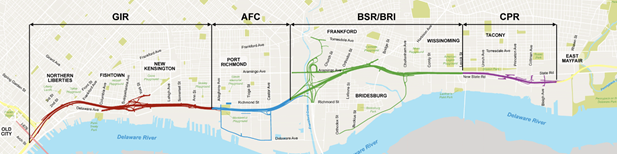
\includegraphics[width=0.8\textwidth]{gfx/chapter-introduction/i95revive_map.png}
	\caption[I-95 Girard Avenue Interchange Stormwater Project.]{I-95 Girard Avenue Interchange Stormwater Project map (PennDOT, 2018).}
	\label{fig:revive-full-map}
\end{figure}

\begin{figure}[ht]
	\centering
	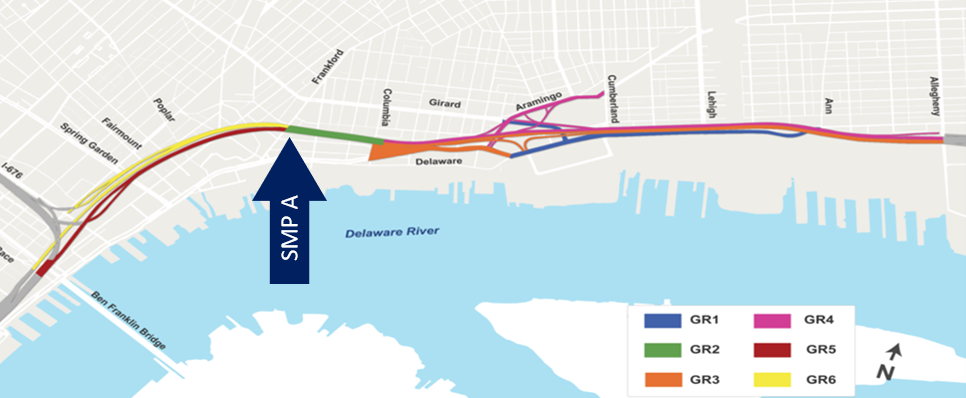
\includegraphics[width=0.8\textwidth]{gfx/chapter-introduction/gr2_map.png}
	\caption[I-95 Girard Avenue Interchange Stormwater Project GIR-GR2 Section.]{I-95 Girard Avenue Interchange Stormwater Project GIR-GR2 section map (PennDOT, 2018).}
	\label{fig:GR2-map}
\end{figure}

SMP A is a linear bioinfiltration type garden nearly 100m in length but only 10-12m wide due to tight urban geometry constraining the site.
Infiltration occurs in over 80\% of the garden, with just a small portion in the center lined to protect neighboring structures.
To better understand the site's hydraulic performance, monitoring equipment was installed in mid-2017 to quantify volume and soil state, and aid in the development of an EPA Stormwater Management Model (SWMM) by former Villanova Center for Resilient Water Systems graduate Elizabeth Calt (\citeyear{Calt2018}).
Further work has been undertaken to improve the monitoring network's reliability and accuracy.
This site is funded by PennDOT through the AECOM University partners program with the goal of investigating the long term performance of GSI as a stormwater management tool.

\section{Research Goals}
The primary goal of this work is to identify multi-faceted strategies for improved long-term monitoring solutions that will enable more thorough analysis of GSI.
The steps outlined in the following chapters are intended to provide insight to PennDOT, AECOM, and their project partners in the continued study of wide-scale GSI projects on the I-95 Girard Avenue Interchange Stormwater Project, as well as to other partners in the city of Philadelphia who seek to expand GSI systems to the watershed scale and beyond.
The creation of more uniform monitoring and long-term analysis practices will help move the design of GSI towards practices that are longer lasting, easier to maintain, and less prone to construction errors or failure.
The steps outlined include three separate facets:
\begin{itemize}
	\item The use of digital sensors with more accurate sensing and data transmission makes continuous monitoring more reliable and less prone to unrecoverable errors.
	\item Storing data in a flexible schema, such as the Stormwater Infrastructure Data Model in use at Villanova, enables long term study and comparison of a multitude of GSI locations.
	\item Event statistics generated from continuous monitoring data, such as recession rate and soil drying rate, can be used to approximate more labor-intensive field and lab tests to ensure continued performance.
\end{itemize}
Each of these topics will be discussed in detail in the following three chapters, with a focus on lessons learned through implementation at SMP A.

